%==========================================
%
% Sibgrapi 2014 paper
% Anderson Rocha, Diego Nehab, ...
%
%==========================================


% Note that the a4paper option is mainly intended so that authors in
% countries using A4 can easily print to A4 and see how their papers will
% look in print - the typesetting of the document will not typically be
% affected with changes in paper size (but the bottom and side margins will).
% Use the testflow package mentioned above to verify correct handling of
% both paper sizes by the user's LaTeX system.
%
% Also note that the "draftcls" or "draftclsnofoot", not "draft", option
% should be used if it is desired that the figures are to be displayed in
% draft mode.
%
\documentclass[10pt, conference]{IEEEtran}
\usepackage[utf8]{inputenc}


% *** MISC UTILITY PACKAGES ***
%
%\usepackage{ifpdf}
% Heiko Oberdiek's ifpdf.sty is very useful if you need conditional
% compilation based on whether the output is pdf or dvi.
% usage:
% \ifpdf
%   % pdf code
% \else
%   % dvi code
% \fi
% The latest version of ifpdf.sty can be obtained from:
% http://www.ctan.org/tex-archive/macros/latex/contrib/oberdiek/
% Also, note that IEEEtran.cls V1.7 and later provides a builtin
% \ifCLASSINFOpdf conditional that works the same way.
% When switching from latex to pdflatex and vice-versa, the compiler may
% have to be run twice to clear warning/error messages.






% *** CITATION PACKAGES ***
%
%\usepackage{cite}
% cite.sty was written by Donald Arseneau
% V1.6 and later of IEEEtran pre-defines the format of the cite.sty package
% \cite{} output to follow that of IEEE. Loading the cite package will
% result in citation numbers being automatically sorted and properly
% "compressed/ranged". e.g., [1], [9], [2], [7], [5], [6] without using
% cite.sty will become [1], [2], [5]--[7], [9] using cite.sty. cite.sty's
% \cite will automatically add leading space, if needed. Use cite.sty's
% noadjust option (cite.sty V3.8 and later) if you want to turn this off.
% cite.sty is already installed on most LaTeX systems. Be sure and use
% version 4.0 (2003-05-27) and later if using hyperref.sty. cite.sty does
% not currently provide for hyperlinked citations.
% The latest version can be obtained at:
% http://www.ctan.org/tex-archive/macros/latex/contrib/cite/
% The documentation is contained in the cite.sty file itself.






% *** GRAPHICS RELATED PACKAGES ***
%
\usepackage{subimages}
\setfigdir{figs}




% *** MATH PACKAGES ***
%
\usepackage[cmex10]{amsmath}
% A popular package from the American Mathematical Society that provides
% many useful and powerful commands for dealing with mathematics. If using
% it, be sure to load this package with the cmex10 option to ensure that
% only type 1 fonts will utilized at all point sizes. Without this option,
% it is possible that some math symbols, particularly those within
% footnotes, will be rendered in bitmap form which will result in a
% document that can not be IEEE Xplore compliant!
%
% Also, note that the amsmath package sets \interdisplaylinepenalty to 10000
% thus preventing page breaks from occurring within multiline equations. Use:
\interdisplaylinepenalty=2500
% after loading amsmath to restore such page breaks as IEEEtran.cls normally
% does. amsmath.sty is already installed on most LaTeX systems. The latest
% version and documentation can be obtained at:
% http://www.ctan.org/tex-archive/macros/latex/required/amslatex/math/
\usepackage{amsthm}
\usepackage{amssymb}
\newtheorem{definition}{Definition}





% *** SPECIALIZED LIST PACKAGES ***
%
%\usepackage{algorithmic}
% algorithmic.sty was written by Peter Williams and Rogerio Brito.
% This package provides an algorithmic environment fo describing algorithms.
% You can use the algorithmic environment in-text or within a figure
% environment to provide for a floating algorithm. Do NOT use the algorithm
% floating environment provided by algorithm.sty (by the same authors) or
% algorithm2e.sty (by Christophe Fiorio) as IEEE does not use dedicated
% algorithm float types and packages that provide these will not provide
% correct IEEE style captions. The latest version and documentation of
% algorithmic.sty can be obtained at:
% http://www.ctan.org/tex-archive/macros/latex/contrib/algorithms/
% There is also a support site at:
% http://algorithms.berlios.de/index.html
% Also of interest may be the (relatively newer and more customizable)
% algorithmicx.sty package by Szasz Janos:
% http://www.ctan.org/tex-archive/macros/latex/contrib/algorithmicx/




% *** ALIGNMENT PACKAGES ***
%
%\usepackage{array}
% Frank Mittelbach's and David Carlisle's array.sty patches and improves
% the standard LaTeX2e array and tabular environments to provide better
% appearance and additional user controls. As the default LaTeX2e table
% generation code is lacking to the point of almost being broken with
% respect to the quality of the end results, all users are strongly
% advised to use an enhanced (at the very least that provided by array.sty)
% set of table tools. array.sty is already installed on most systems. The
% latest version and documentation can be obtained at:
% http://www.ctan.org/tex-archive/macros/latex/required/tools/


%\usepackage{mdwmath}
%\usepackage{mdwtab}
% Also highly recommended is Mark Wooding's extremely powerful MDW tools,
% especially mdwmath.sty and mdwtab.sty which are used to format equations
% and tables, respectively. The MDWtools set is already installed on most
% LaTeX systems. The lastest version and documentation is available at:
% http://www.ctan.org/tex-archive/macros/latex/contrib/mdwtools/


% IEEEtran contains the IEEEeqnarray family of commands that can be used to
% generate multiline equations as well as matrices, tables, etc., of high
% quality.


%\usepackage{eqparbox}
% Also of notable interest is Scott Pakin's eqparbox package for creating
% (automatically sized) equal width boxes - aka "natural width parboxes".
% Available at:
% http://www.ctan.org/tex-archive/macros/latex/contrib/eqparbox/



% *** PDF, URL AND HYPERLINK PACKAGES ***
%
\usepackage{hyperref}





% *** Do not adjust lengths that control margins, column widths, etc. ***
% *** Do not use packages that alter fonts (such as pslatex).         ***
% There should be no need to do such things with IEEEtran.cls V1.6 and later.
% (Unless specifically asked to do so by the journal or conference you plan
% to submit to, of course. )


% correct bad hyphenation here
\hyphenation{op-tical net-works semi-conduc-tor}


\begin{document}
%
% paper title
% can use linebreaks \\ within to get better formatting as desired
\title{Example of IEEEtran.cls, adapted for Sibgrapi 2014}

%------------------------------------------------------------------------- 
% change the % on next lines to produce the final camera-ready version 
\newif\iffinal
%\finalfalse
\finaltrue
\newcommand{\jemsid}{99999}
%------------------------------------------------------------------------- 

% author names and affiliations
% use a multiple column layout for up to two different
% affiliations

%\iffinal
%  \author{%
%    \IEEEauthorblockN{John Silva, Jo{\~a}o Smith}
%    \IEEEauthorblockA{%
%      line 1 (of Affiliation): dept. name of organization\\
%      line 2: name of organization, acronyms acceptable\\
%      line 3: City, Country\\
%      line 4: Web page: \href{http://www.institution1.eud/~firstauthor}{www.institution1.eud/$\sim$\{john,joao\}}}
%  \and
%    \IEEEauthorblockN{Authors Name/s per 2nd Affiliation}
%    \IEEEauthorblockA{%
%      line 1 (of Affiliation): dept. name of organization\\
%      line 2: name of organization, acronyms acceptable\\
%      line 3: City, Country\\
%      line 4: Email:  \href{mailto:name@xyz.com}{name@xyz.com}}
%  }
%\else
%  \author{Sibgrapi paper ID: \jemsid \\ }
%\fi

% for over three affiliations, or if they all won't fit within the width
% of the page, use this alternative format:
% 
\author{\IEEEauthorblockN{Leandro Botelho\IEEEauthorrefmark{1},
Augusto Cunha e
Thales Vieira}
\IEEEauthorblockA{Universidade Federal de Alagoas\\
\IEEEauthorrefmark{1}Instituto de Computação,
Instituto de Matemática\\
Maceió, Alagoas.}}


%------------------------------------------------------------------------- 
% Special Sibgrapi teaser
\teaser{%
  \oneimage{Teasing result of our method: from this data input (left), the relevant feature are extracted using our technique (middle), producing effective result (right).}{.99}{teaser.pdf}
}
%------------------------------------------------------------------------- 



% make the title area
\maketitle



%==========================================
\begin{abstract}
A edição de superfícies suaves representadas por malhas de triângulos no computador é uma área ativa 
de pesquisa em Modelagem Geométrica, devido à sua gama cada vez maior de aplicações na indústria 
e no desenho artístico. Porém, a variedade de ferramentas de edição de superfícies disponíveis atualmente 
ainda é escassa. Problemas como deformação de forma livre, inserção de texturas geométricas, inpainting, 
reconstrução com restrições, remoção de ruído, reparos, entre outras, carecem de métodos robustos, 
flexíveis e eficientes que permitam edição interativa e que sejam capazes de reconstruir superfícies de 
qualidade. 
Neste trabalho, usamos a representação de superfícies baseada no operador gradiente discreto 
da malha, para desenvolver novas ferramentas interativas de edição de objetos 3d representados por malhas 
de triângulos.

% DO NOT USE SPECIAL CHARACTERS, SYMBOLS, OR MATH IN YOUR TITLE OR ABSTRACT.
%
\end{abstract}

\begin{IEEEkeywords}
one or two words; separated by semicolon; from specific; to generic fields;

\end{IEEEkeywords}


\IEEEpeerreviewmaketitle


% Wherever Times is specified, Times Roman or Times New Roman may be used. If neither is available on your system, please use the font closest in appearance to Times. Avoid using bit-mapped fonts if possible. True-Type 1 or Open Type fonts are preferred. Please embed symbol fonts, as well, for math, etc.

%==========================================
%==========================================


%==========================================
\section{Introdução}
%
Representação e processamento de objetos 3d é um dos mais importantes tópicos em Computação 
Gráfica e Modelagem Geométrica. A maneira como um objeto 3d é definido restringe o conjunto de 
operações que podem ser aplicadas a ele. Diferentes representações de objetos podem exibir diferentes 
propriedades geométricas, combinatórias e até perceptivas da forma. 
Uma das representações de superfícies mais pesquisadas nos últimos anos é a que se baseia no 
operador gradiente discreto em malhas triangulares. Esta representação fornece intrinsicamente as 
propriedades geométricas destas superfícies, e tem sido muito utilizada para resolver problemas de 
edição, onde destacamos [1].

No problema de edição de superfícies, deseja-se transformar uma superfície suave, representada no 
computador por uma malha de triângulos, em uma outra superfície, preservando características como 
continuidade, suavidade, detalhes, e ao mesmo tempo respeitando restrições impostas pelo usuário. A 
Figura 1 ilustra o problema.

Porém, a variedade de ferramentas de edição de superfícies disponíveis atualmente ainda é escassa. 
Problemas como deformação de forma livre, inserção de texturas geométricas, inpainting, reconstrução 
com restrições, remoção de ruído, reparos, entre outras, carecem de métodos robustos, flexíveis e 
eficientes que permitam edição interativa e que sejam capazes de reconstruir superfícies de qualidade. 
No projeto precedente, o operador Laplaciano e gradiente discreto foram estudados, e uma 
implementação computacional da equação de Poisson foi desenvolvida. Neste projeto, as propriedades do 
operador gradiente serão investigadas para o desenvolvimento de novas ferramentas de edição interativas 
de objetos 3d representados por malhas de triângulos. Estas ferramentas serão inspiradas na equação de 
Poisson, já adotada com sucesso para edição de imagens em [2].


%------------------------------------------------------------------------- 
\paragraph*{Contribuições}
%
[THALES ALTERE AQUI]


%------------------------------------------------------------------------- 
%\subsection{Related work}
%%
%We can roughly classify the approaches used for our application in three categories: first category, second category, and last category.\\
%Approaches in the first category were introduced by Pierre~\cite{Sibgrapi2014} using this and that techniques.
%
%
%\subimages[htb]{Technique overview}{overview}{%
%  \subimage[First step]{.31}{overviewa}%
%  \subimage[Second step]{.31}{overviewb}%
%  \subimage[Result]{.31}{overviewc}%
%}


%==========================================
%\subsection{Technique overview}
\subsection{Trabalhos Relacionados}

Para o desenvolvimento desse nosso trabalho, percebemos que métodos de edição de superfícies têm uma participação forte na área de Modelagem Geométrica. Podemos visualizar esse tipo de atividade em aplicações envolvendo indústrias ou manipulação de desenhos artísticos.

Durante muitos anos, a abordagem utilizada na literatura, envolvia uma representação baseada em superfícies paramétricas \cite{FarinG}, que podem ter uma generalização para domínios de base não regular usando técnicas de subdivisão \cite{SCHRZORI}.

Com o crescimento da divulgação dos Scanners 3D, a obtenção de geometrias de superfícies de objetos reais ficou acessível \cite{NEUGEBAUER}. Porém, esses novos tipos de superfícies apresentam uma amostragem densa e não suave, não sendo os métodos de edição de superfícies já existentes. Devido à isso, houve o surgimentos de novas ferramentas para edição desses tipos de superfícies .

Diversos métodos, surgiram até então para deformação de superfícies. Para o estado da arte dos métodos variacionais lineares, temos  \cite{Olga}, principalmente em relação métodos baseados no operador Laplaciano discreto \cite{Lang} e o Operador Gradiente Discreto \cite{Yu:2004}; que são versões adaptadas para superfícies diferenciadas, para malhas de triângulos.

Por fim, destacamos diversos problemas de edição que carecem de alternativas robustas e interativas. Ao nosso trabalho, a base de autovetores da matriz laplaciana de superfície é usada para realizar edição por meio de frequências.

\subsection{Visão Geral}

Ao longo do desenvolvimento de nosso trabalho, inicialmente utilizamos uma estrutura \cite{che05} capaz de manter as informações de geometria, topologia e conectividade de vértices, arestas e faces de uma malha triangular que representa uma superfícies bidimensional no espaço euclidiano.

%-------------- Tenho que pegar a imagem do retalho triangular ---------------------





Para desenvolver esse tipo de ferramentas, focamos na Equação de Poisson

\begin{eqnarray}
\bigtriangleup x' = div\  \textbf{$g_x$}
\end{eqnarray}










%
%In order to produce this application, we start with this processing, followed by this technique. In order to cope with this challenge, we introduce this formulation to produce this intermediate result. The formulation leads to this type of system, which is efficiently solved by adapting this technique. The final result is produced by this transform. The whole process is schematized in 
\figref{overview}.



%==========================================
\section{Technical background}
%
In this section, we detail this classical technique. The reader can find a more complete exposition in the work of Paul~\cite{Sibgrapi2014}.


%------------------------------------------------------------------------- 
\subsection{Important concept}
%
An \emph{important concept} is a type of object:
\begin{definition}[Important concept]
Given this and that, an object $X$ is an important concept if it respects the following properties\ldots{}
\end{definition}


%------------------------------------------------------------------------- 
\subsection{Usual adaptation}
%
This concept has been used for applications similar to ours~\cite{Sibgrapi2014}, using the following formulation\ldots{}
%==========================================
%\section{New technique or technique adaptation}
\section{Alinhamento Semi - automático}
\label{sec:technique}

\subsection{Iterative Closest Point}

Um dos grandes problemas no desenvolvimento de reconstrução de malhas, com certeza se caracteriza pelo alinhamento de duas malhas parcialmente sobrepostas; com dados pontos iniciais correspondentes para uma relativa transformação.

Para nos auxiliar no problema de alinhamento em relação às duas malhas, utilizamos o algoritmo \textit{Iterative Closest Point} (ICP) \cite{Zhang:1994}; que nos fornece à minimização da distância de cada ponto de uma malha D, a cada ponto correspondente de cada malha M.

\subsection{Iterative Closest Point}

Um dos grandes problemas no desenvolvimento de reconstrução de malhas, com certeza se caracteriza pelo alinhamento de duas malhas parcialmente sobrepostas; com dados pontos iniciais correspondentes para uma relativa transformação.

Para nos auxiliar no problema de alinhamento em relação às duas malhas, utilizamos o algoritmo \textit{Iterative Closest Point} (ICP) \cite{Zhang:1994}; que nos fornece à minimização da distância de cada ponto de uma malha D, a cada ponto correspondente de cada malha M.

Para o nosso problema, utilizamos um conjunto de passos para resolve-los. Inicialmente escolhemos nosso conjunto de vertíces de uma malha M, que apresenta seu respectivo correspondente à malha D; Segue \ref{ICP} como imagem. Após esse passo, utilizamos o cálculo dos centroides em relação à cada malha. Em seguida, desenvolvemos o cálculo do alinhamento, aonde envolvemos os principais operadores de transformação(rotação e translação, respectivamente) em relação à cada conjunto de correspondências entre M e D, na qual nos retorna uma matriz de transformação; e por fim aplicamos o alinhamento, utilizando a matriz de transformação em relação à malha que sofre a sobreposição.

\begin{figure}[h]
\center
    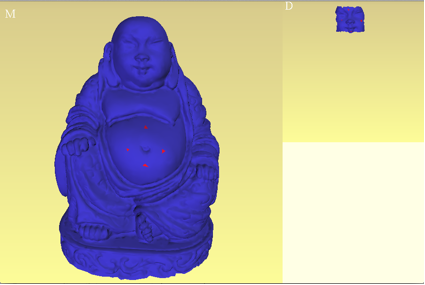
\includegraphics[width=8cm]{ImagemICP2}
        \label{ICP}
\end{figure}
\vspace{4mm}

\subsection{Parametrização conforme}

Para nos facilitar na classificação do método de parametrização, utilizamos uma técnica de bordo livre, com foco em deformação para análise complexa. Com isso, aplicamos a parametrização espectral de \cite{Mullen} nas duas malhas, mantendo como restrição que os vértices correspondentes sejam mapeados para as mesmas coordenadas paramétricas.

%$\mathbb{R}^{3} \longrightarrow \mathbb{R}^2$,
Para isso, inicialmente aplicamos uma projeção em ambas malhas no intuito de encontrar o menor eixo do \textit{bounding box}, e "prender" os vértices extremos.
 
Posteriormente, utilizamos uma técnica conhecida como LSCM (\textit{Least Squares Conformal Maps}) \cite{Levy:2002}; que tem o objetivo em minimizar a energia conforme, devido as superfícies em geral não admitirem parametrização conforme.

A minimização M se caracteriza pela seguinte equação:
\[ M = \sum_{T}= \left|\left| \left[ \begin{array}{c}  \dfrac{\partial v}{\partial x} \\ \\  \dfrac{\partial v}{\partial y}  \end{array} \right] - \left[ \begin{array}{c}  -\dfrac{\partial u}{\partial y}  \\ \\ \dfrac{\partial u}{\partial x}  \end{array} \right] \right| \right|^{2} \]
\vspace*{0.3mm}

Mantendo dois vértices para determinar a rotação, translação e escalonamento.

E por fim. aplicamos um algoritmo, conhecido como \textit{Thin Plane Spline} \cite{Duchon} que nos favorece a interpolação necessária para formação da parametrização 2D.
%
%Our technique aims at obtaining that result. It particularly suits to the problem since it is formulated as\ldots{}


%%------------------------------------------------------------------------- 
%\subsection{Formulation}
%
%
%%------------------------------------------------------------------------- 
%\subsection{Solution}
%
%
%%------------------------------------------------------------------------- 
%\subsection{Initialization and tuning}
%==========================================
\section{Reconstrução}
%
Após a seleção das correspondências entre a malha principal e a malha do detalhe a ser
adicionada e as parametrizações já estarem alinhadas, iremos trabalhar apendas com as parametrizaçãos
no $\mathbb{R}^2$. Definimos o conjunto de half-edges do bordo da malha detalhe como 
$B = {he_0, he_1, he_2, \ldots, he_n} | \forall n \in \mathbb{N}: O(he_n) = -1$, onde $O( )$ retorna o oposto da
half-edge $HE_n$, $-1$ se não existir e o indice do oposto caso exista, também definimos a poligonal
$P = {v_0, v_1, v_2, ..., v_n} | \forall n \in \mathbb{N}: v_n = vertex(HE_n)$, onde $vertex( )$ retorna o vertice
da half-edge. 

Sendo assim iremos excluir cada triângulo da parametrização da malha principal que intersecta ou é
interior à $P$. Com isso observamos a criação de um componente conexo como podemos ver na [figura 4.1],
assim precisamos triangular o espaço entre as parametrizações. Para isto vamos usar uma triangulação com
restrições.

%------------------------------------------------------------------------- 
\subsection{Triangulação com Restrições}
%
Usaremos a técnica de sweeping(varreduda) para realizar a triangulação, obedecendo o conjunto das
arestas da restrição $E = {e_0, e_1, e_2, \ldots, e_n} | \forall n \in \mathbb{N}: e_n$ é uma aresta da restrição,
ou seja, é uma aresta que deve fazer parte da nova triangulação.

%------------------------------------------------------------------------- 
\subsection{Equação de Poisson}
%==========================================
\section{Resultados}
%
We performed the above-mentioned experiments on the following type of data: \ldots{} For each data, we used the following tuning parameters of our method.


\begin{table}
\caption{Performances results: timings are expressed in milliseconds.}
\label{tab:perfs}
\centering
\begin{tabular}{lr|rr|c}
\multicolumn{1}{c}{\bf Data} &
\multicolumn{1}{c|}{\bf Size} &
\multicolumn{1}{c}{\bf Ours} &
\multicolumn{1}{c|}{\bf Previous} &
\multicolumn{1}{c}{\bf Gain} \\ \hline
Data 1	&        50 	& 0.1 &     1 000	& x$10^3$ \\
Data 2	&      100 	& 0.2 &     2 000	& x$10^3$ \\
Data 3	&      500 	& 0.8 &   10 000	& x$10^3$ \\
Data 4	&   1 000 	& 1.2 &   20 000	& x$10^3$ \\
Data 5	&   5 000 	& 1.9 & 100 000	& x$10^4$ \\
Data 6	& 10 000 	& 2.1 & 200 000	& x$10^4$
\end{tabular}
\end{table}
%
%------------------------------------------------------------------------- 
\subsection{Performances}
%
We report on Table~\ref{tab:perfs} the performances of our technique on a computer at xxGhz with this graphic card.
We observe that our technique outperforms previous approaches on this kind of data, and an equivalent result on this other kind of data.

\subimages[htb]{Quality assessment}{quality}{
  \subimage{.48}{qualitya}%
  \subimage{.48}{qualityb}%
}


%------------------------------------------------------------------------- 
\subsection{Quality}
%
As observed on \figref{quality}, our method achieve good results in this situation. 
This can be measured by this criterion, and the results are reported on Table~\ref{tab:quality}.

\begin{table}
\caption{Quality measures: timings are expressed in milliseconds.}
\label{tab:quality}
\centering
\begin{tabular}{l|r|r}
\multicolumn{1}{c}{\bf Images} &
\multicolumn{1}{c|}{\bf PSNR} &
\multicolumn{1}{c}{\bf  MSE} \\ \hline
Image 1	&  40.2	& 0.02 \\
Image 2	&  30.9	& 1.02 \\
Image 3 &  20.1 & 0.18 \\
\end{tabular}
\end{table}


%------------------------------------------------------------------------- 
\subsection{Limitation}
%
As mentioned in Section~\ref{sec:technique}, we expect our method to suit better this kind of data. On the other kind, this particularity does not fit into our formulation for this and that reason. Indeed, this can be observed in the results of \figref{quality}. 
We plan to improve for that kind of data in future work. However, our technique performed well on this data, which does not respect our condition, since this other aspect reduced the negative impact of its characteristic.
%==========================================
\section{Conclusion}
%
In this paper, we introduced this technique and showed that it is particularly appropriate for that application. We obtained this and that improvements, and plan to extend this application in that direction in future work.
%==========================================
\iffinal
% use section* for acknowledgement
\section*{Acknowledgment}
%
The authors would like to thank this colleague and this financing institute.
\fi



%==========================================

% trigger a \newpage just before the given reference
% number - used to balance the columns on the last page
% adjust value as needed - may need to be readjusted if
% the document is modified later
%\IEEEtriggeratref{8}
% The "triggered" command can be changed if desired:
%\IEEEtriggercmd{\enlargethispage{-5in}}

\bibliographystyle{IEEEtran}
\bibliography{example}

%\emph{SIBGRAPI 2014, Proceedings of the XXVII Brazilian Symposium on Computer Graphics and Image Processing}.\hskip 1em plus 0.5em minus 0.4em\relax  Rio de Janeiro, Brazil: {IEEE}, August 2014.

\end{document}
